% Paso 2 c) y d) (Anderson).
\appendix
\section*{Anexos}
\addcontentsline{toc}{section}{Anexos}

\subsection*{Anexo A. Lista de referencias IEEE exportada}
\addcontentsline{toc}{subsection}{Anexo A. Lista de referencias IEEE exportada}
% Paso 2 c): la lista exportada desde Zotero o Mendeley.

\subsection*{Anexo B. Biblioteca en el gestor de referencias}
\addcontentsline{toc}{subsection}{Anexo B. Biblioteca en el gestor de referencias}
% Paso 2 d): captura de pantalla de la biblioteca. Guardarla en figuras/ y quitar el comentario.
% \begin{figure}[h]
%   \centering
%   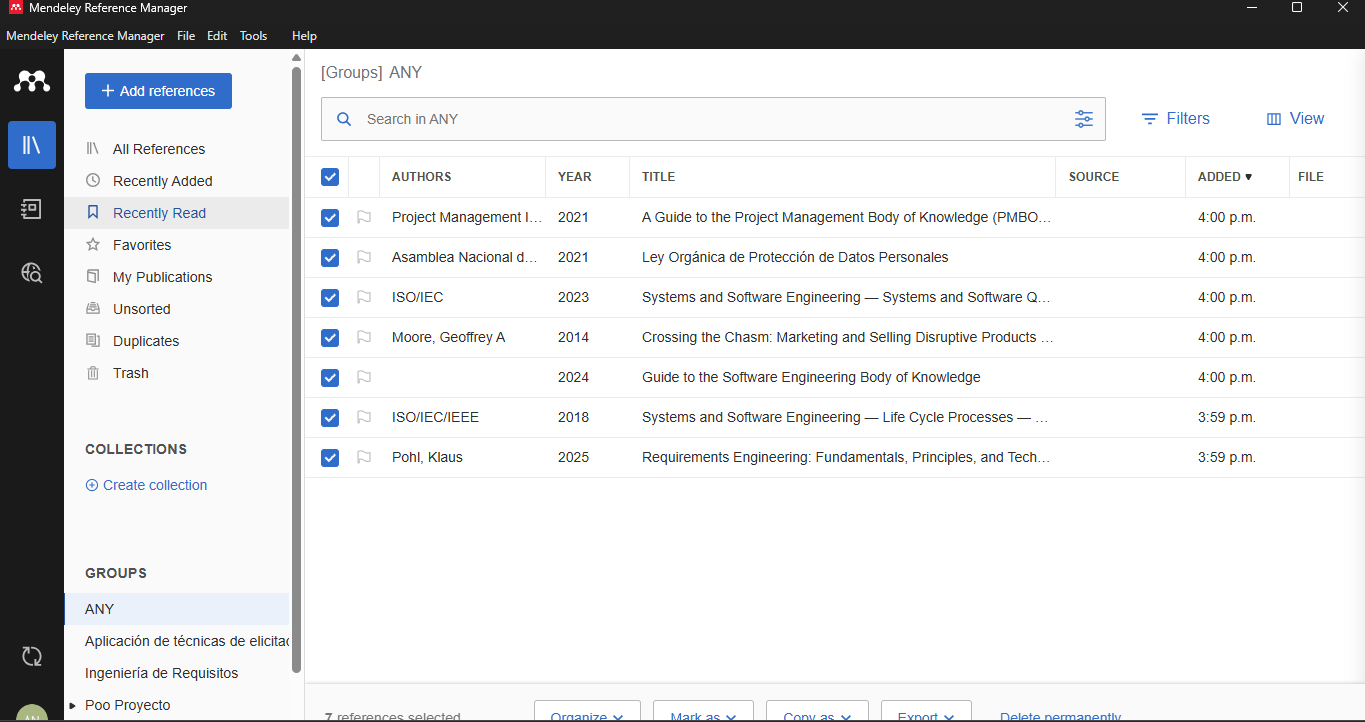
\includegraphics[width=\textwidth]{figuras/biblioteca_zotero.png}
%   \caption{Biblioteca de referencias en el gestor}
% \end{figure}
